\section{Control Plots}
\label{sec:control}

In order to validate the Monte Carlo simulations, we produce data/Monte Carlo comparison plots (control plots) of the light jets control region (JCR, 0 medium b-tagged jets) and of the signal region (SR), both blinded in the $115 < \Mgg < 130$ GeV region.  
In order for background and data to match, the DiPhoton+Jets contribution has been scaled by a factor of 1.5, while the prompt-fake and fake-fake contributions from the GJets and QCD samples have been scaled to data. 
It should be stated that the background MC is not used at any time in this analysis. 
The signal in these plots is normalized for $500$ fb.


\begin{figure*}[thb]
  \centering
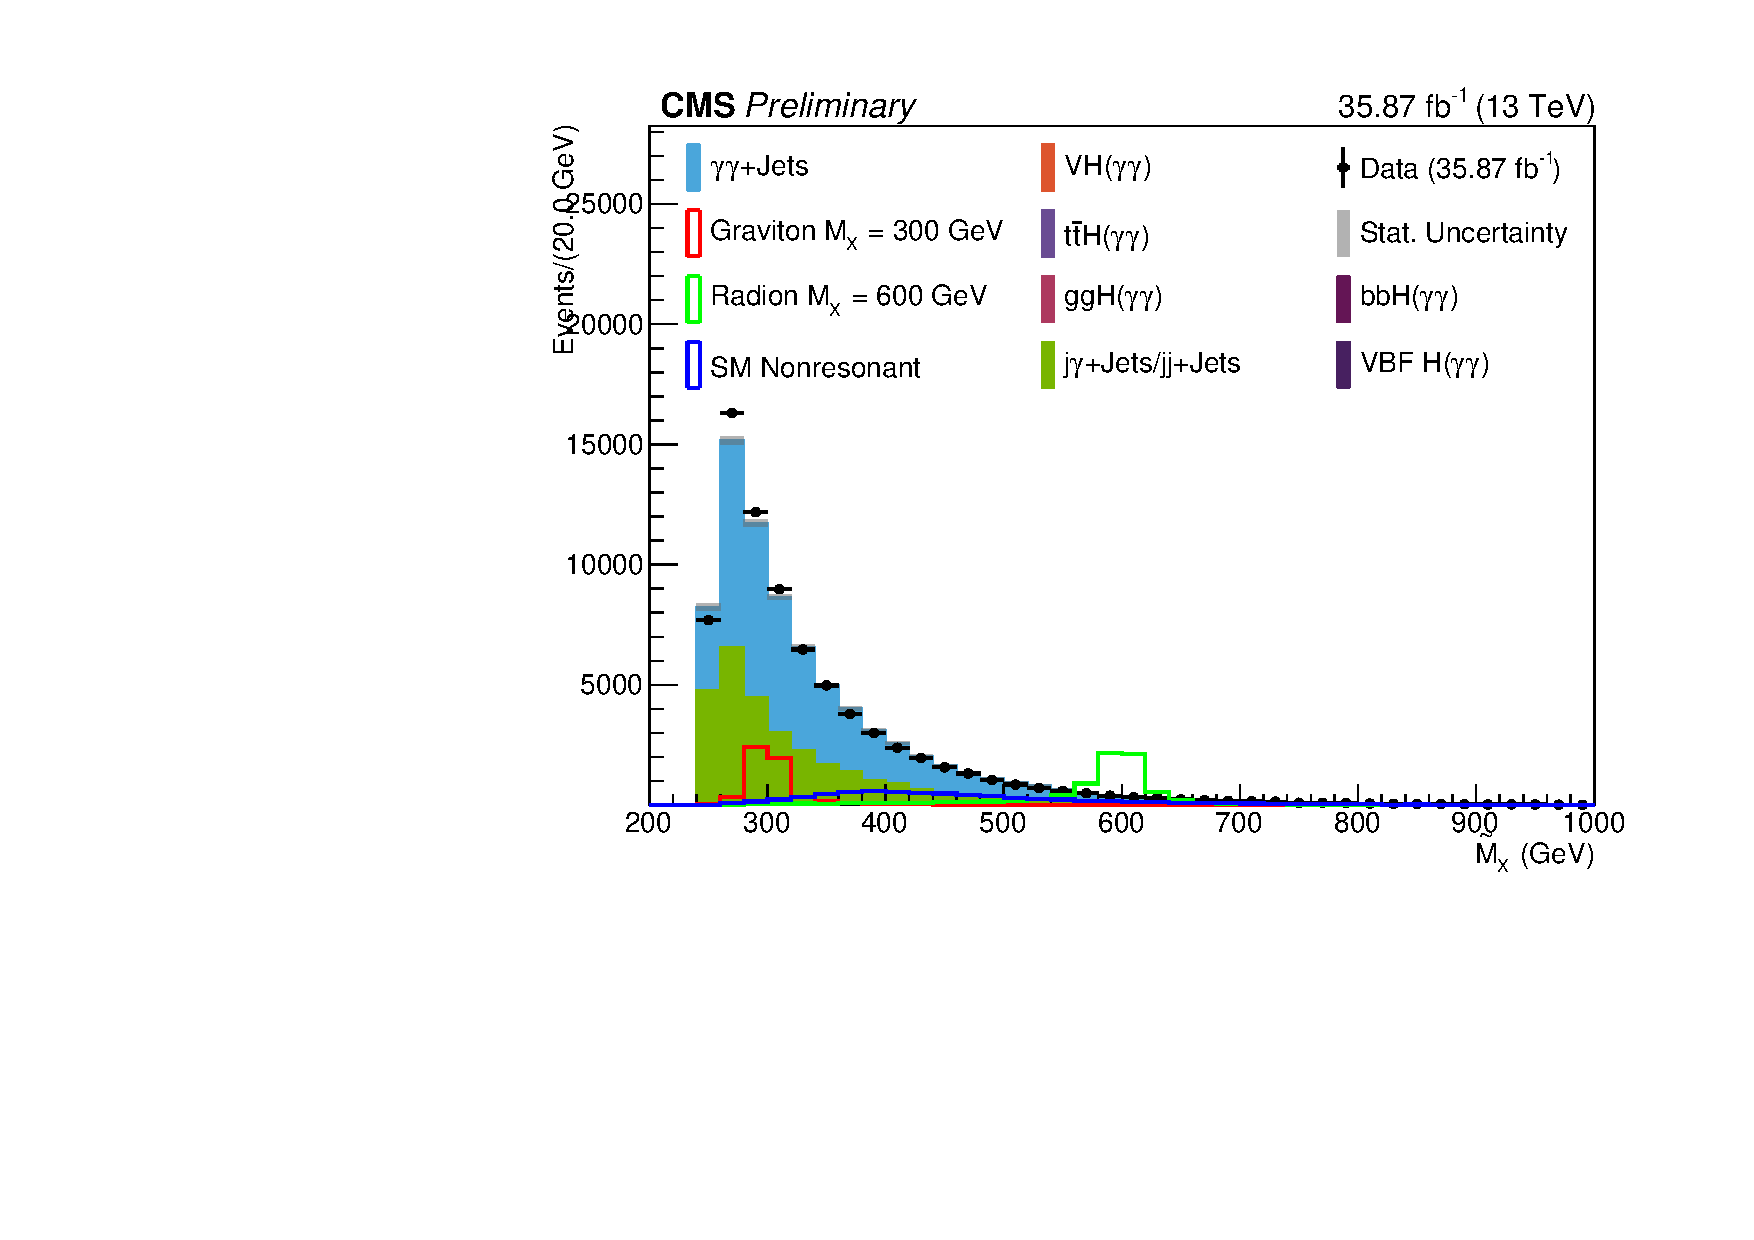
\includegraphics[width=0.45\textwidth]{figures/sec-control/NP_MXprime.pdf}\hfil
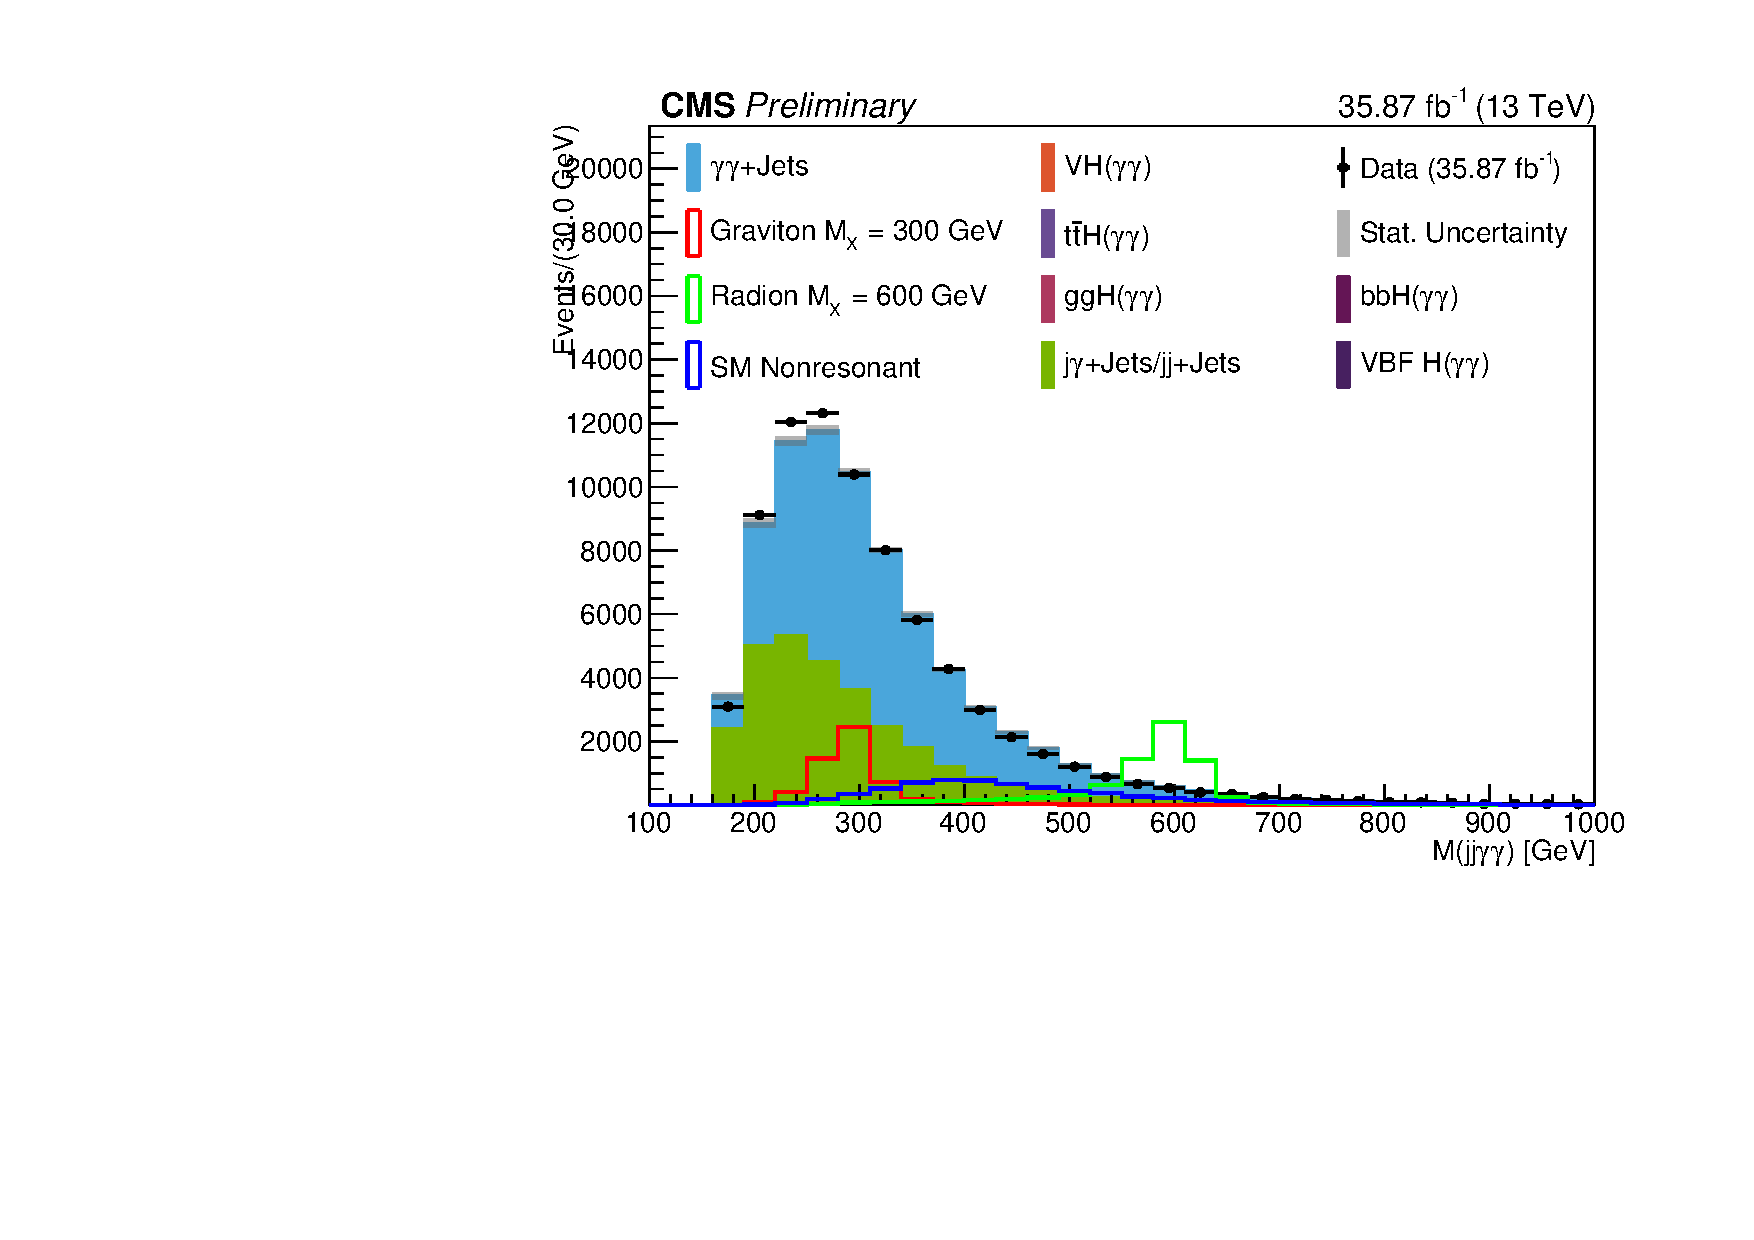
\includegraphics[width=0.45\textwidth]{figures/sec-control/NP_dicandidate_Mass.pdf}\hfil
  \caption{Distributions for the blinded signal region.}
\label{fig:cp_mgg1}
\end{figure*}
\begin{figure*}[thb]
  \centering
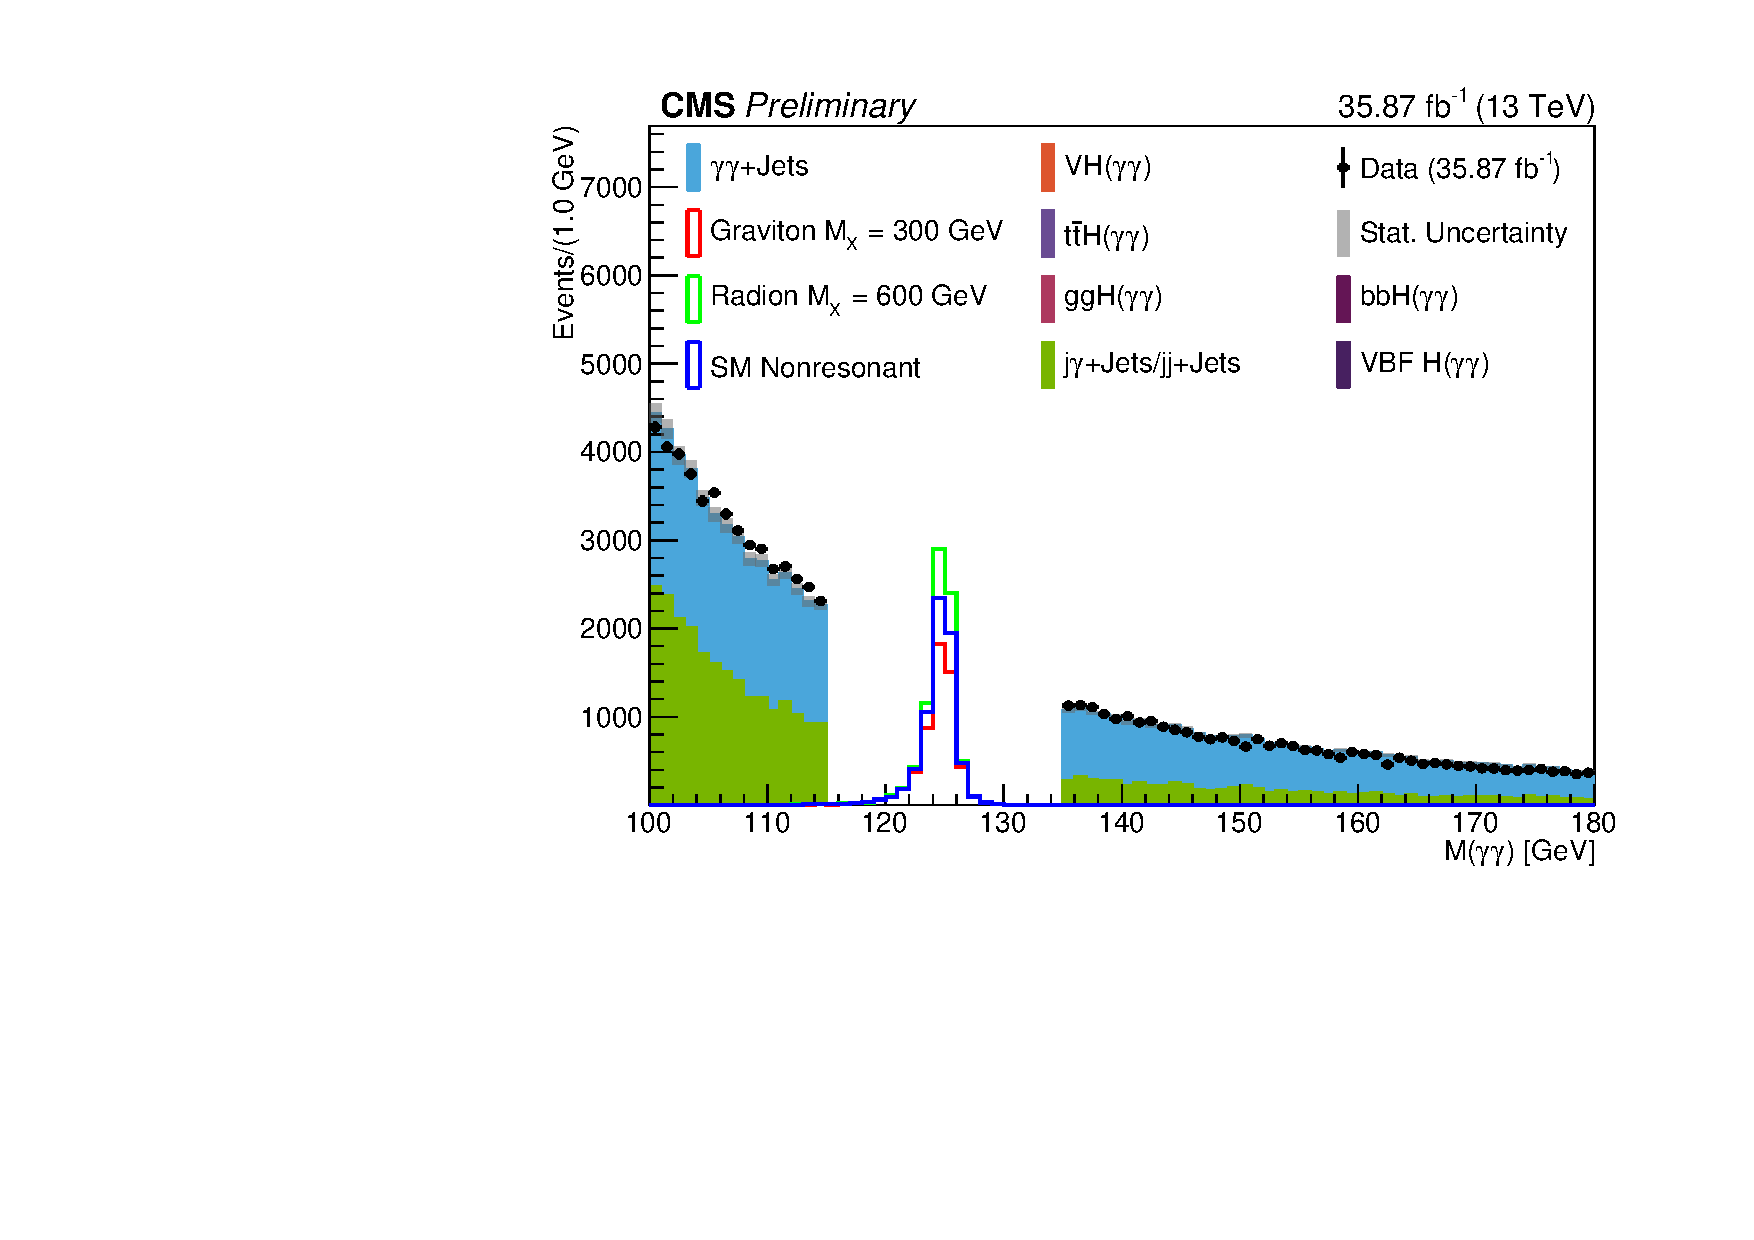
\includegraphics[width=0.45\textwidth]{figures/sec-control/NP_diPho_Mass.pdf}\hfil
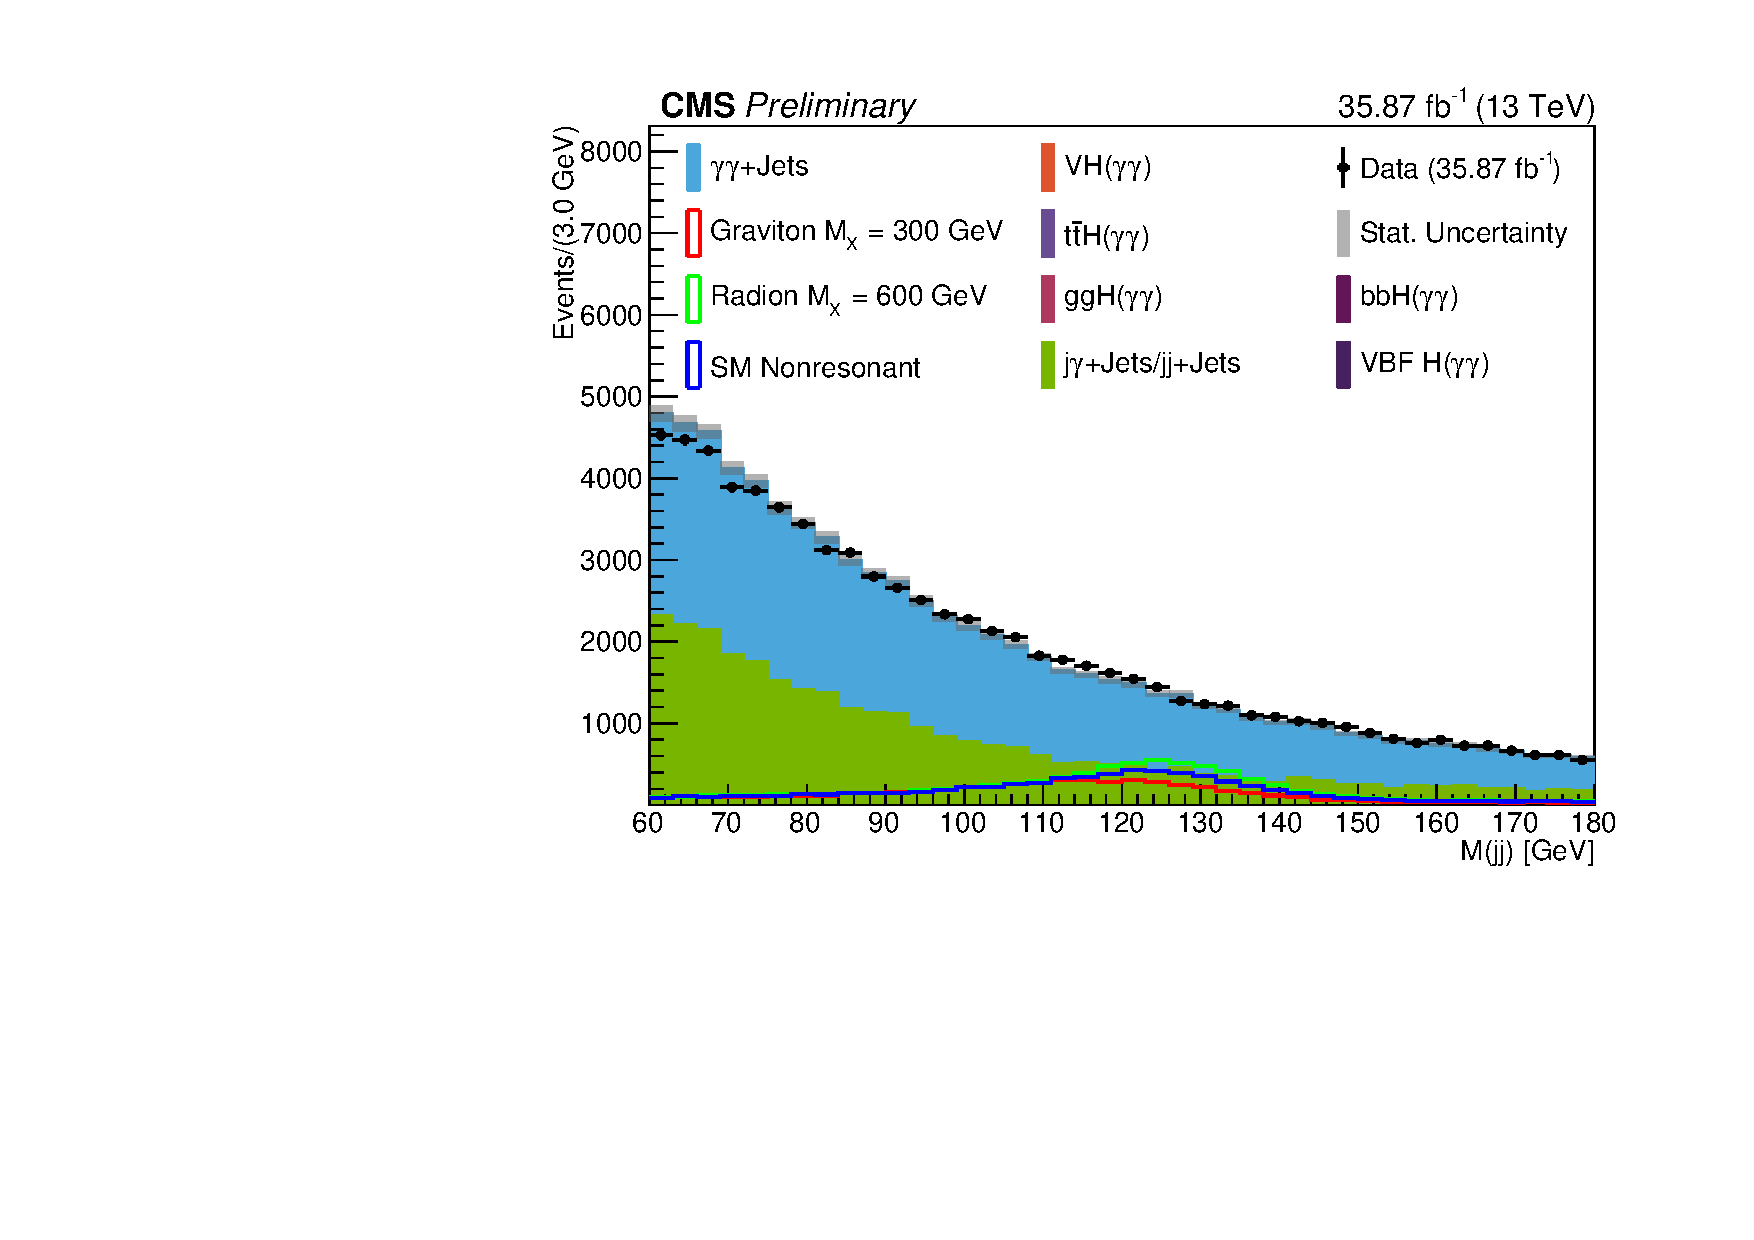
\includegraphics[width=0.45\textwidth]{figures/sec-control/NP_diJet_Mass.pdf}\hfil
  \caption{Distributions for the blinded signal region.}
\label{fig:cp_mgg2}
\end{figure*}
\begin{figure*}[thb]
  \centering
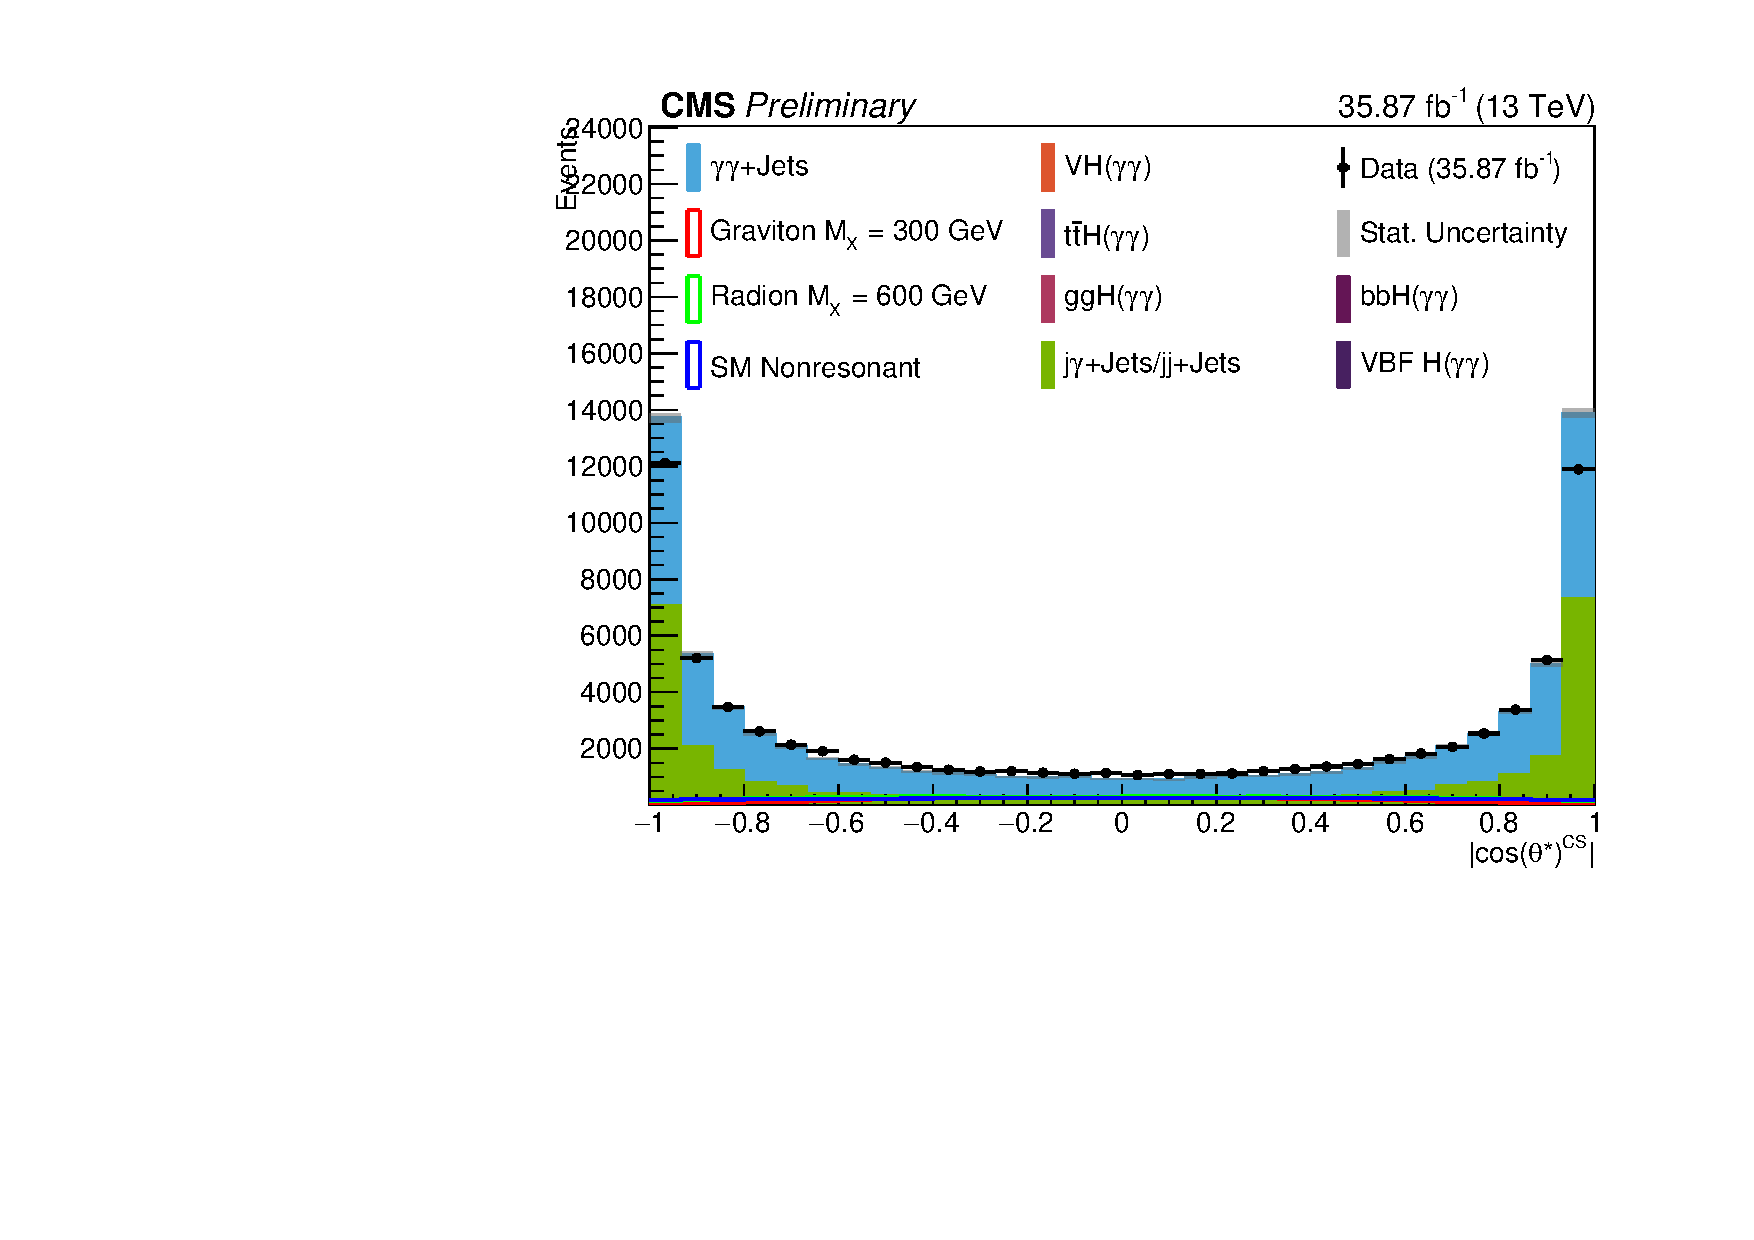
\includegraphics[width=0.45\textwidth]{figures/sec-control/NP_CosThetaStar_CS.pdf}\hfil
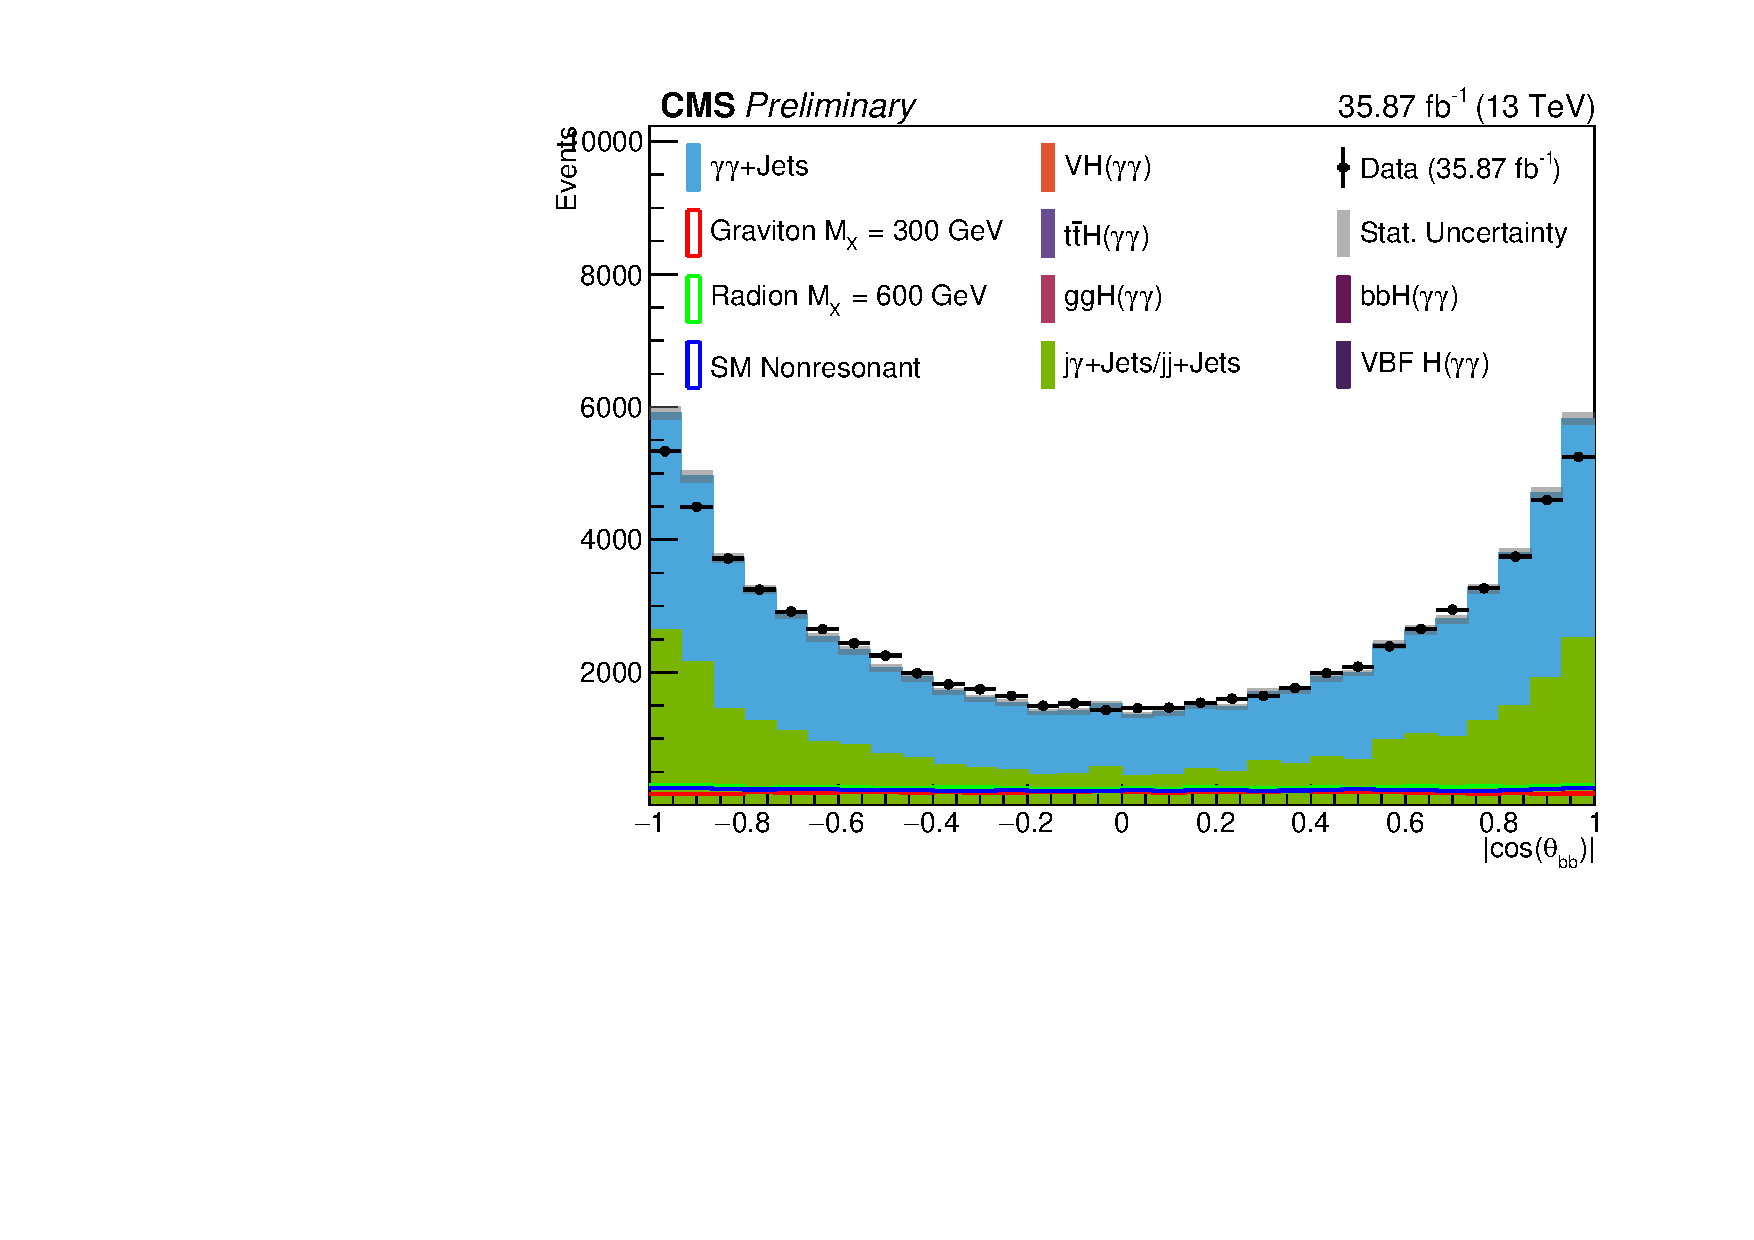
\includegraphics[width=0.45\textwidth]{figures/sec-control/NP_CosTheta_bb.pdf}\hfil
  \caption{Distributions for the blinded signal region.}
\label{fig:cp_mgg3}
\end{figure*}
\begin{figure*}[thb]
  \centering
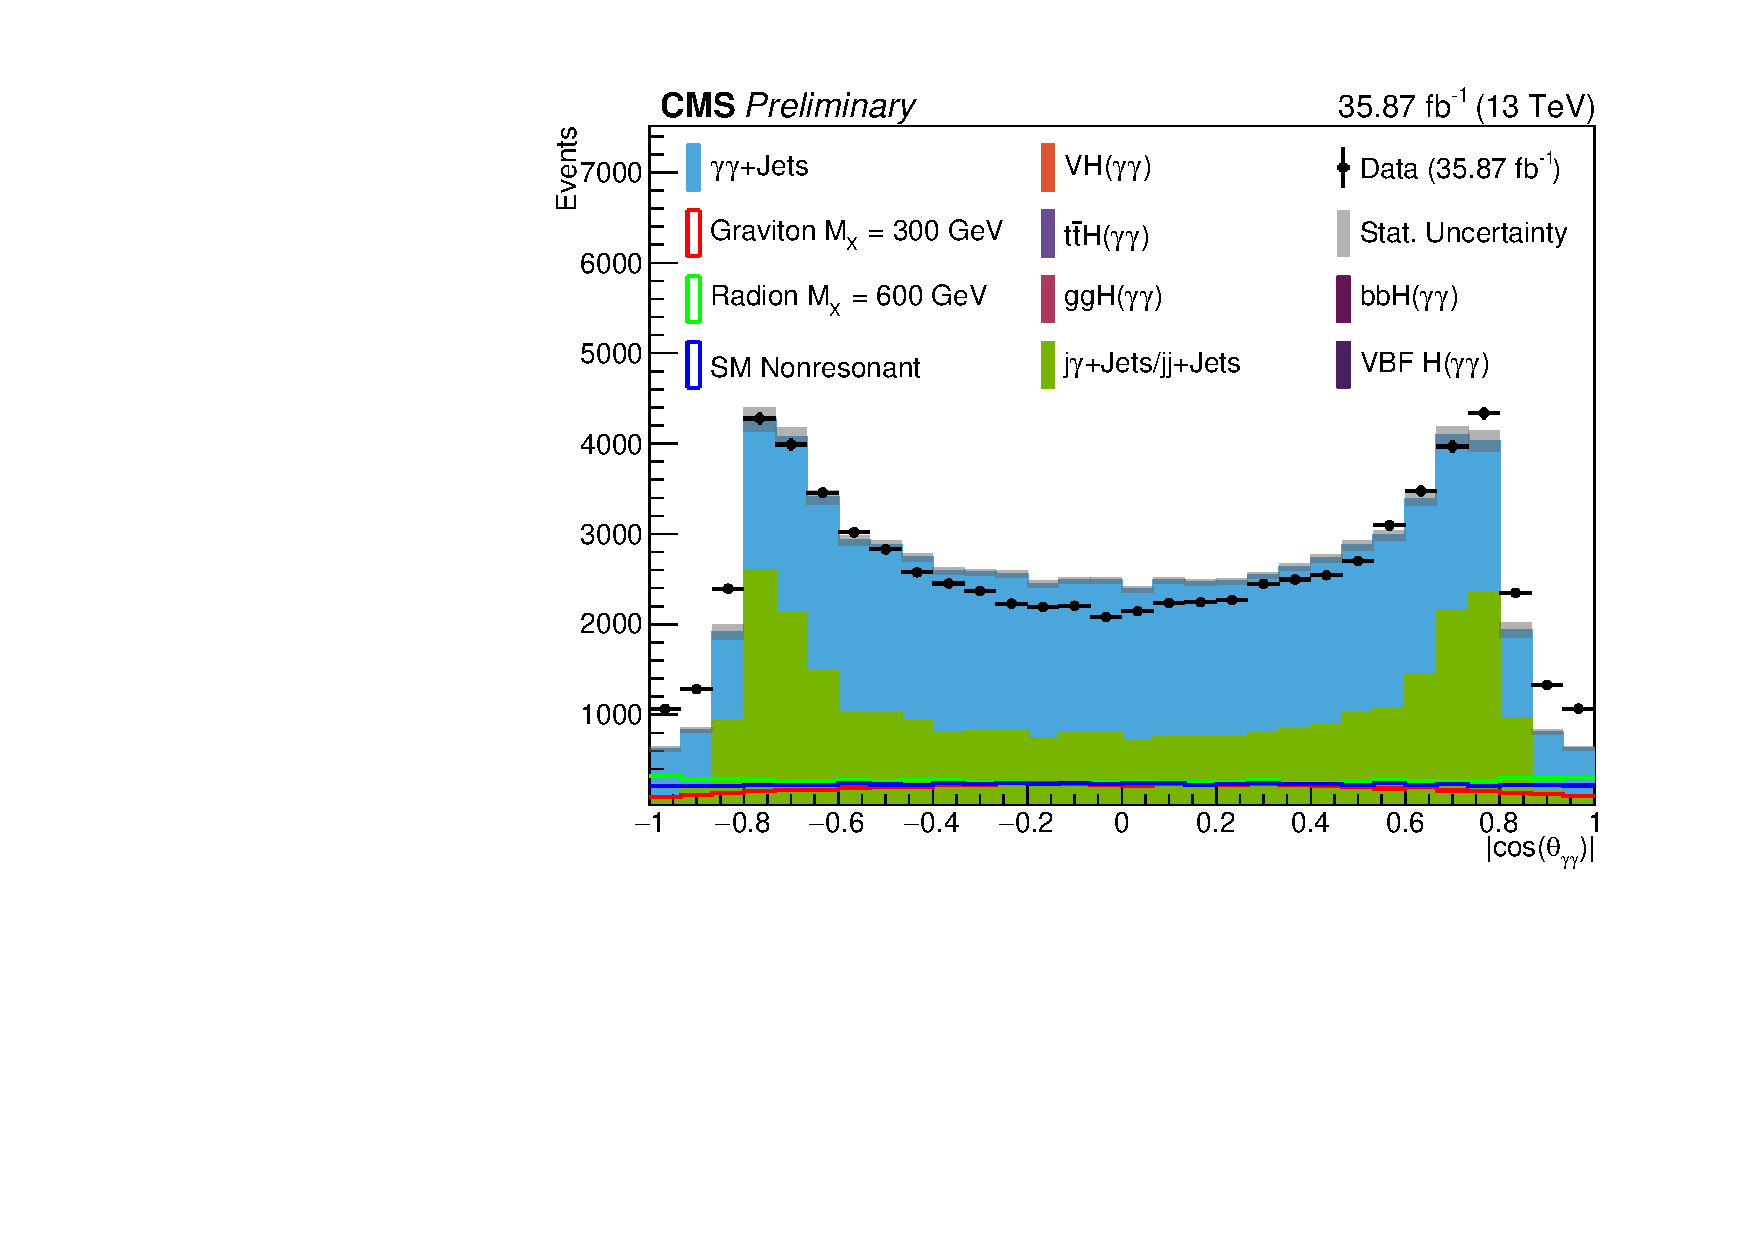
\includegraphics[width=0.45\textwidth]{figures/sec-control/NP_CosTheta_gg.pdf}\hfil
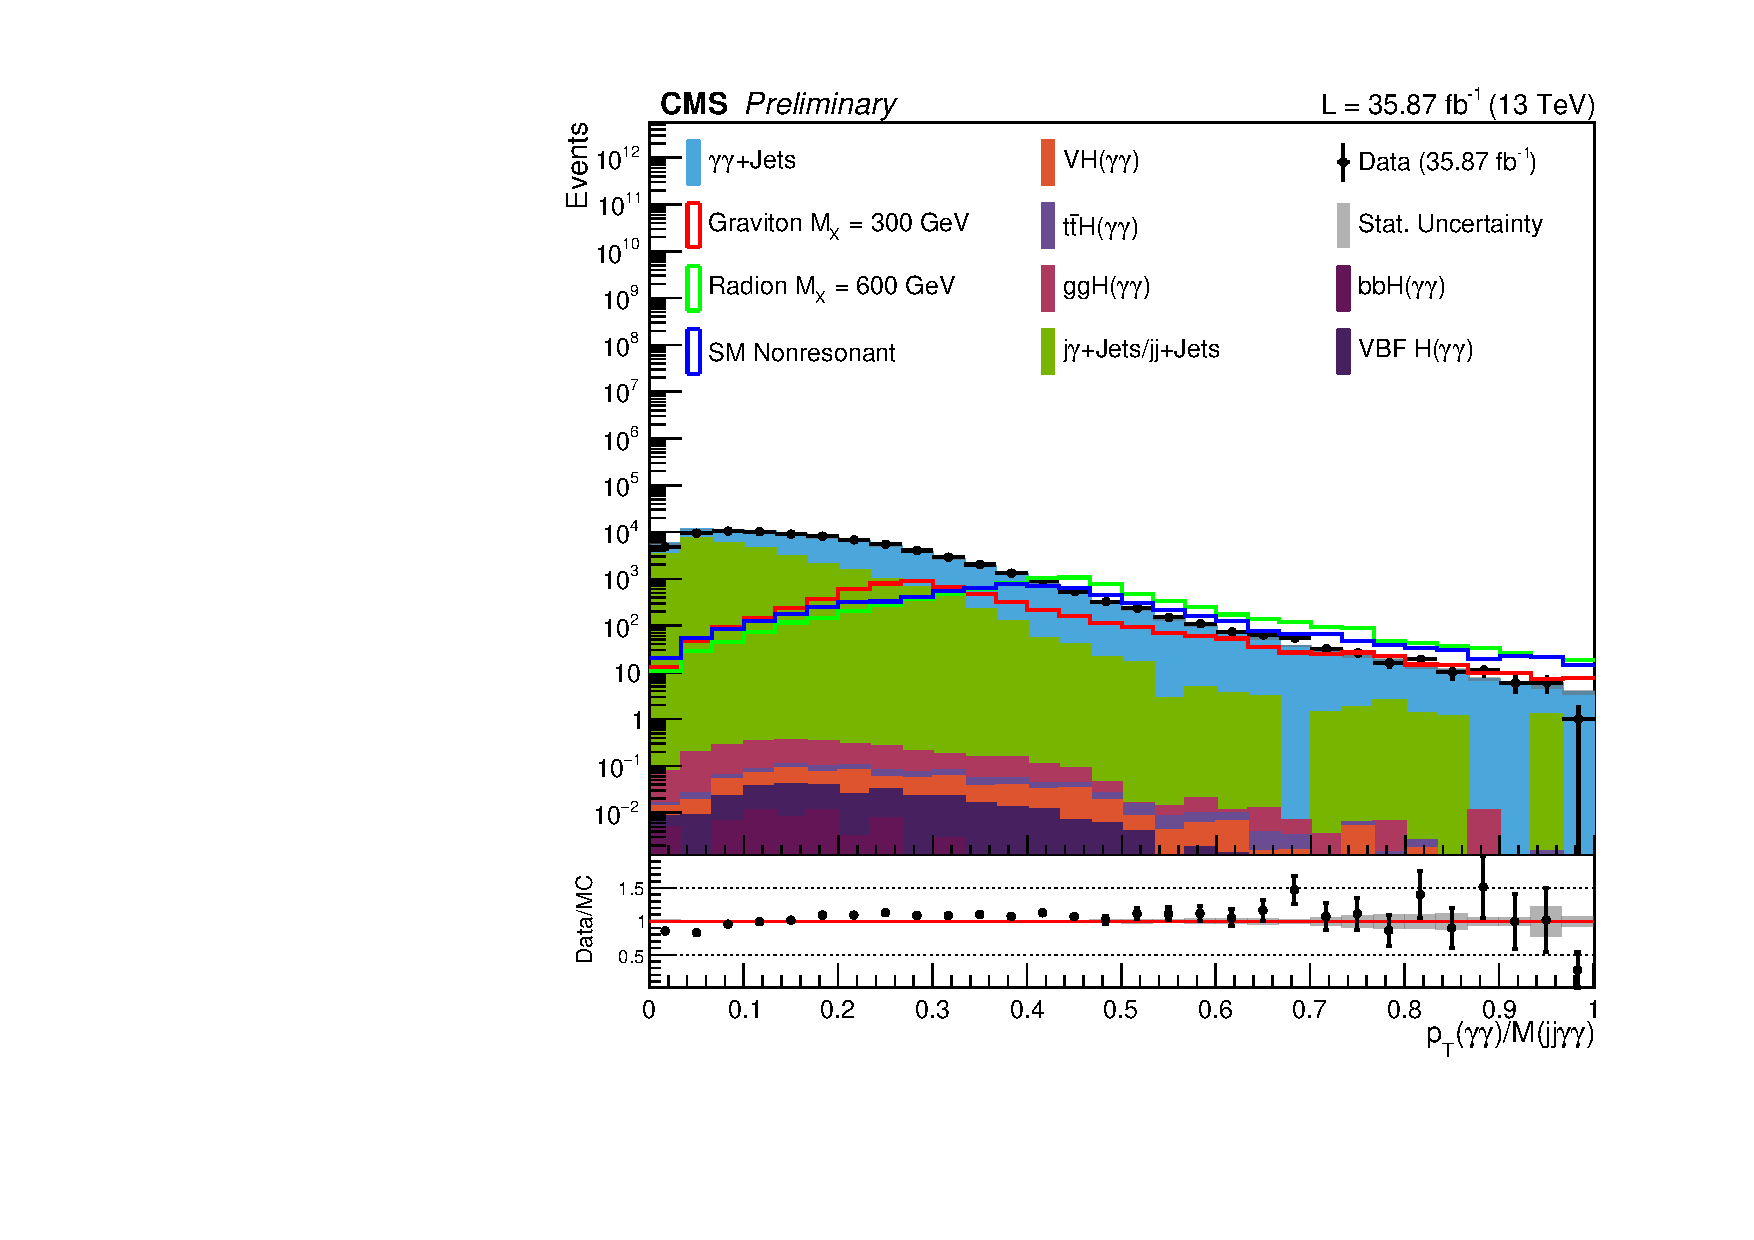
\includegraphics[width=0.45\textwidth]{figures/sec-control/LOG_ggptmjjgg.pdf}\hfil
  \caption{Distributions for the blinded signal region.}
\label{fig:cp_mgg4}
\end{figure*}
\begin{figure*}[thb]
  \centering
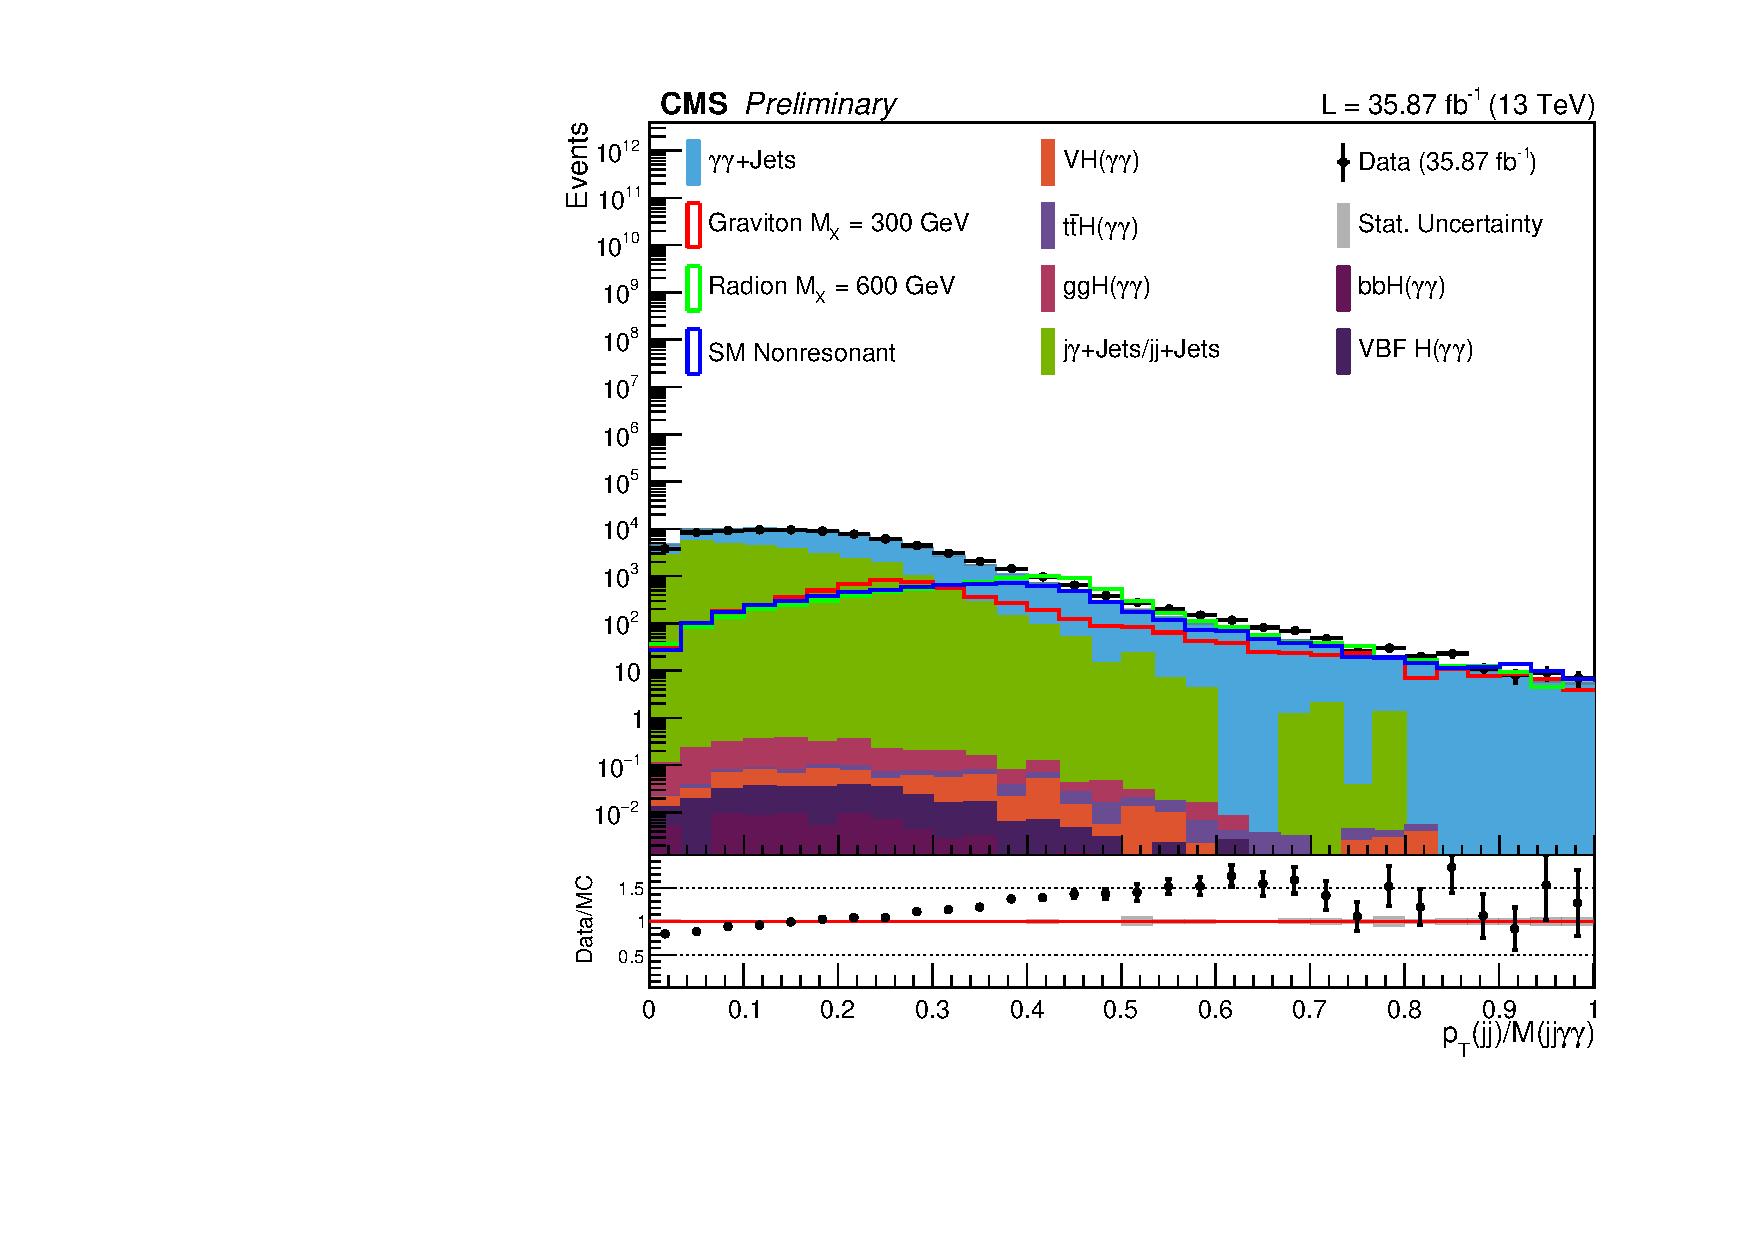
\includegraphics[width=0.45\textwidth]{figures/sec-control/LOG_jjptmjjgg.pdf}\hfil
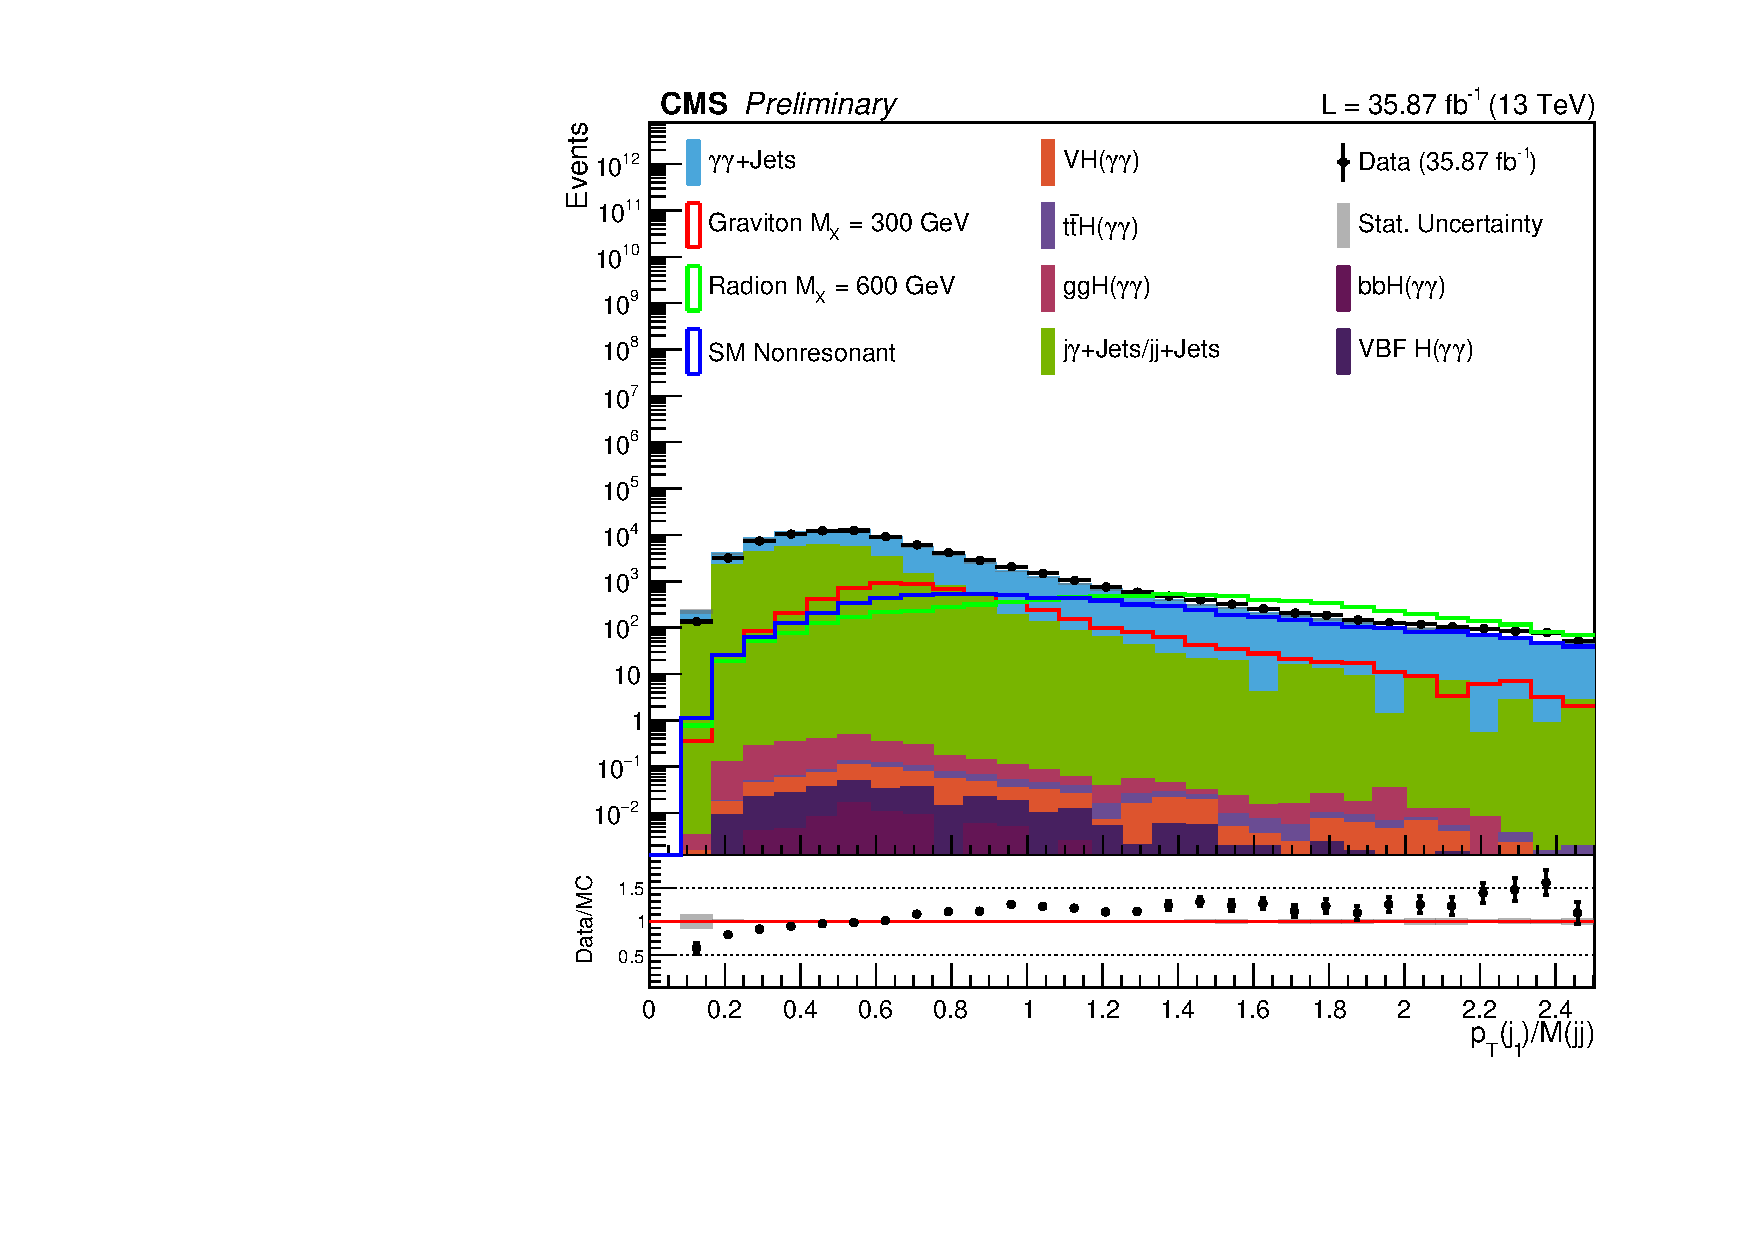
\includegraphics[width=0.45\textwidth]{figures/sec-control/LOG_ljetptmgg}\hfil
  \caption{Distributions for the blinded signal region.}
\label{fig:cp_mgg5}
\end{figure*}
\begin{figure*}[thb]
  \centering
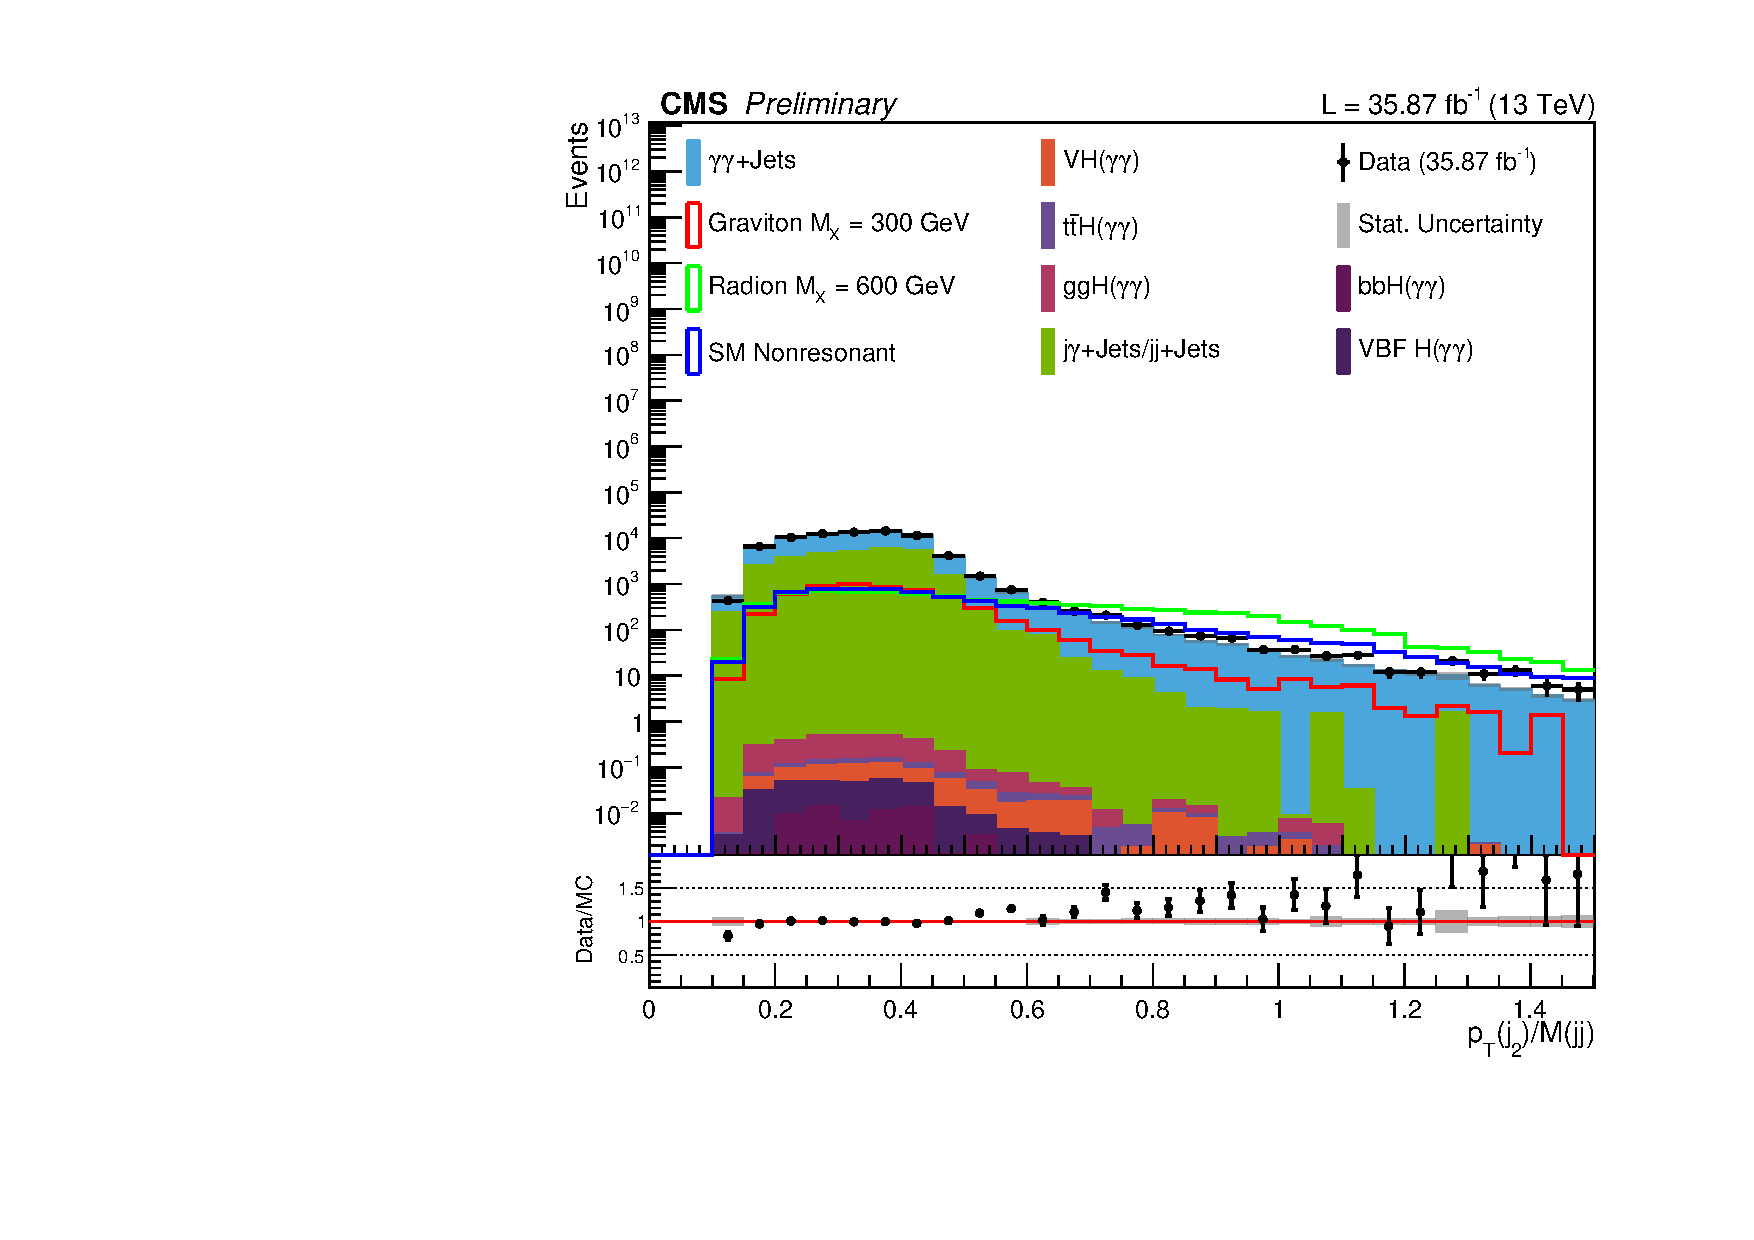
\includegraphics[width=0.45\textwidth]{figures/sec-control/LOG_sjetptmgg}\hfil
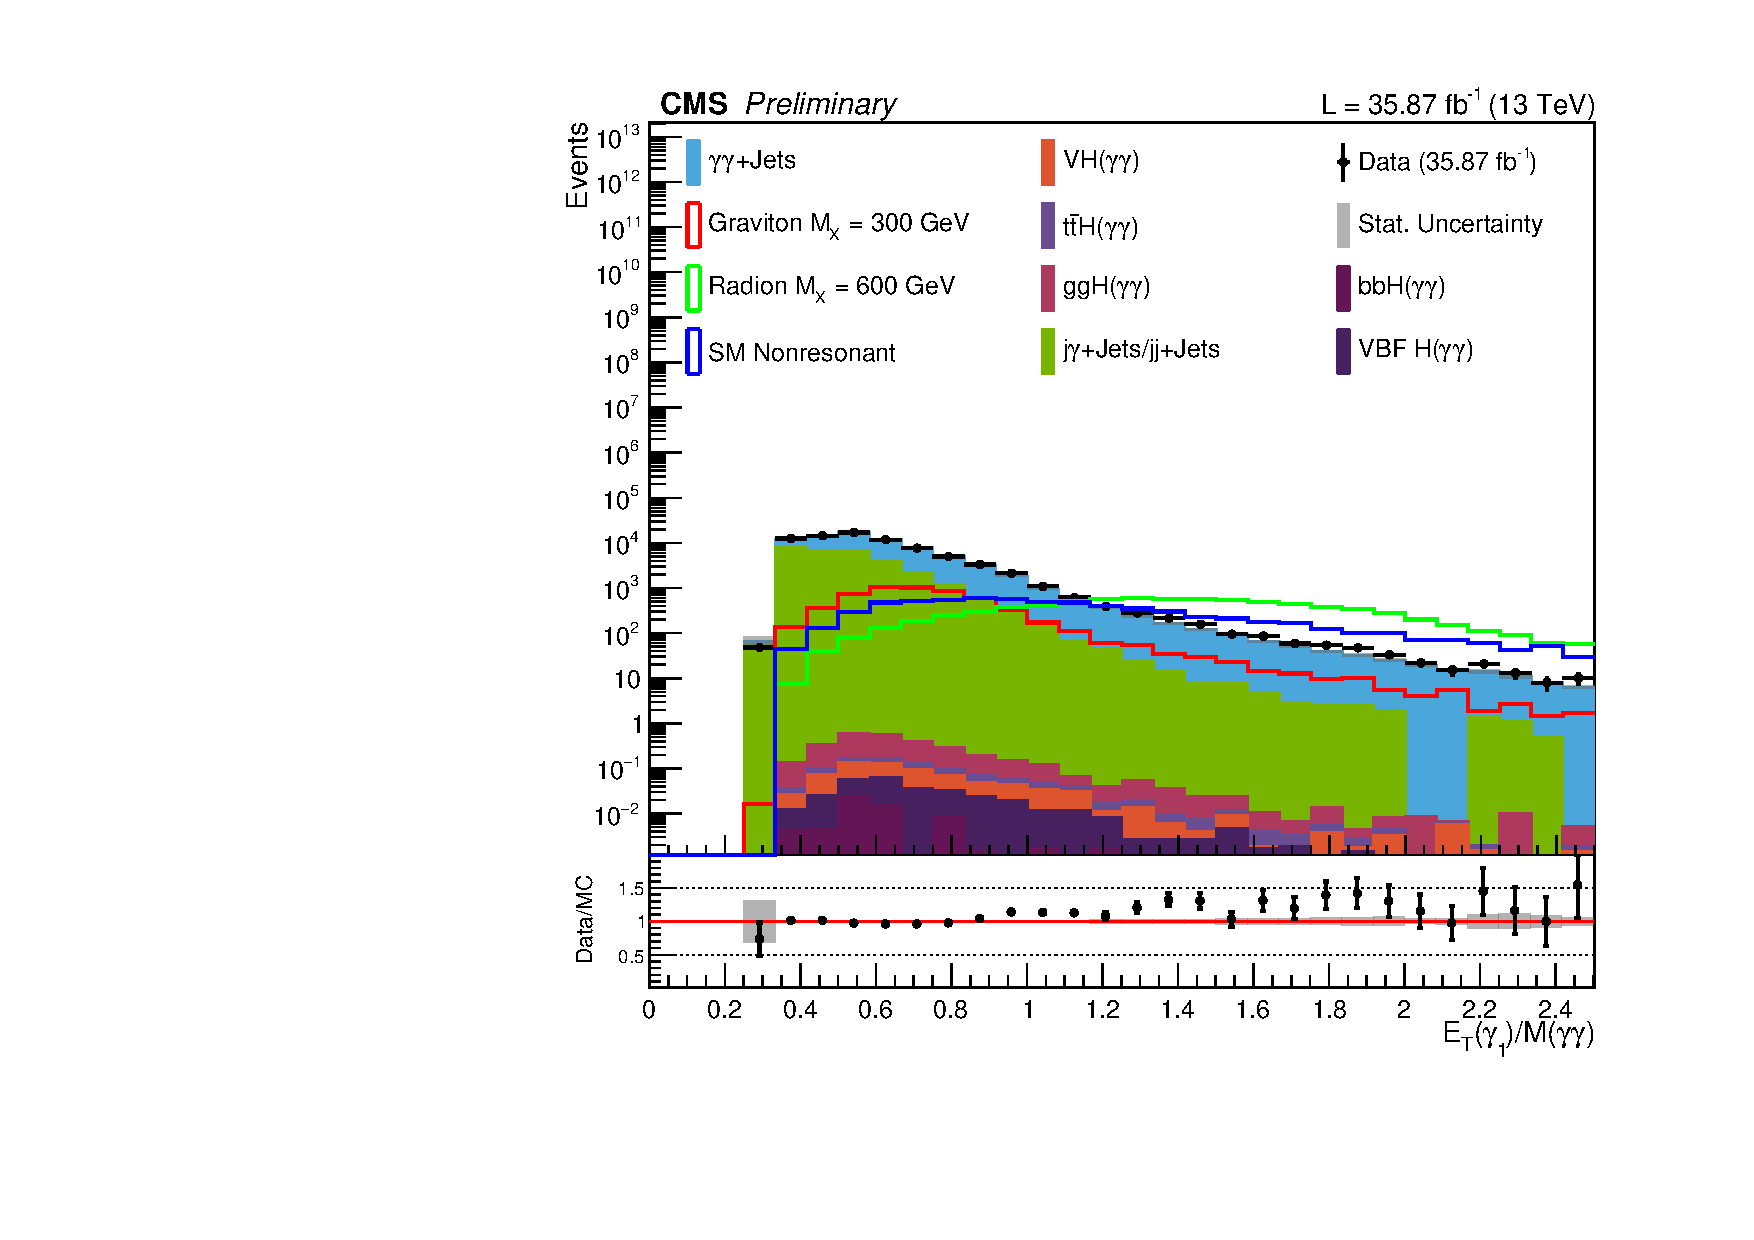
\includegraphics[width=0.45\textwidth]{figures/sec-control/LOG_lphoptmgg}\hfil
  \caption{Distributions for the blinded signal region.}
\label{fig:cp_mgg6}
\end{figure*}
\begin{figure*}[thb]
  \centering
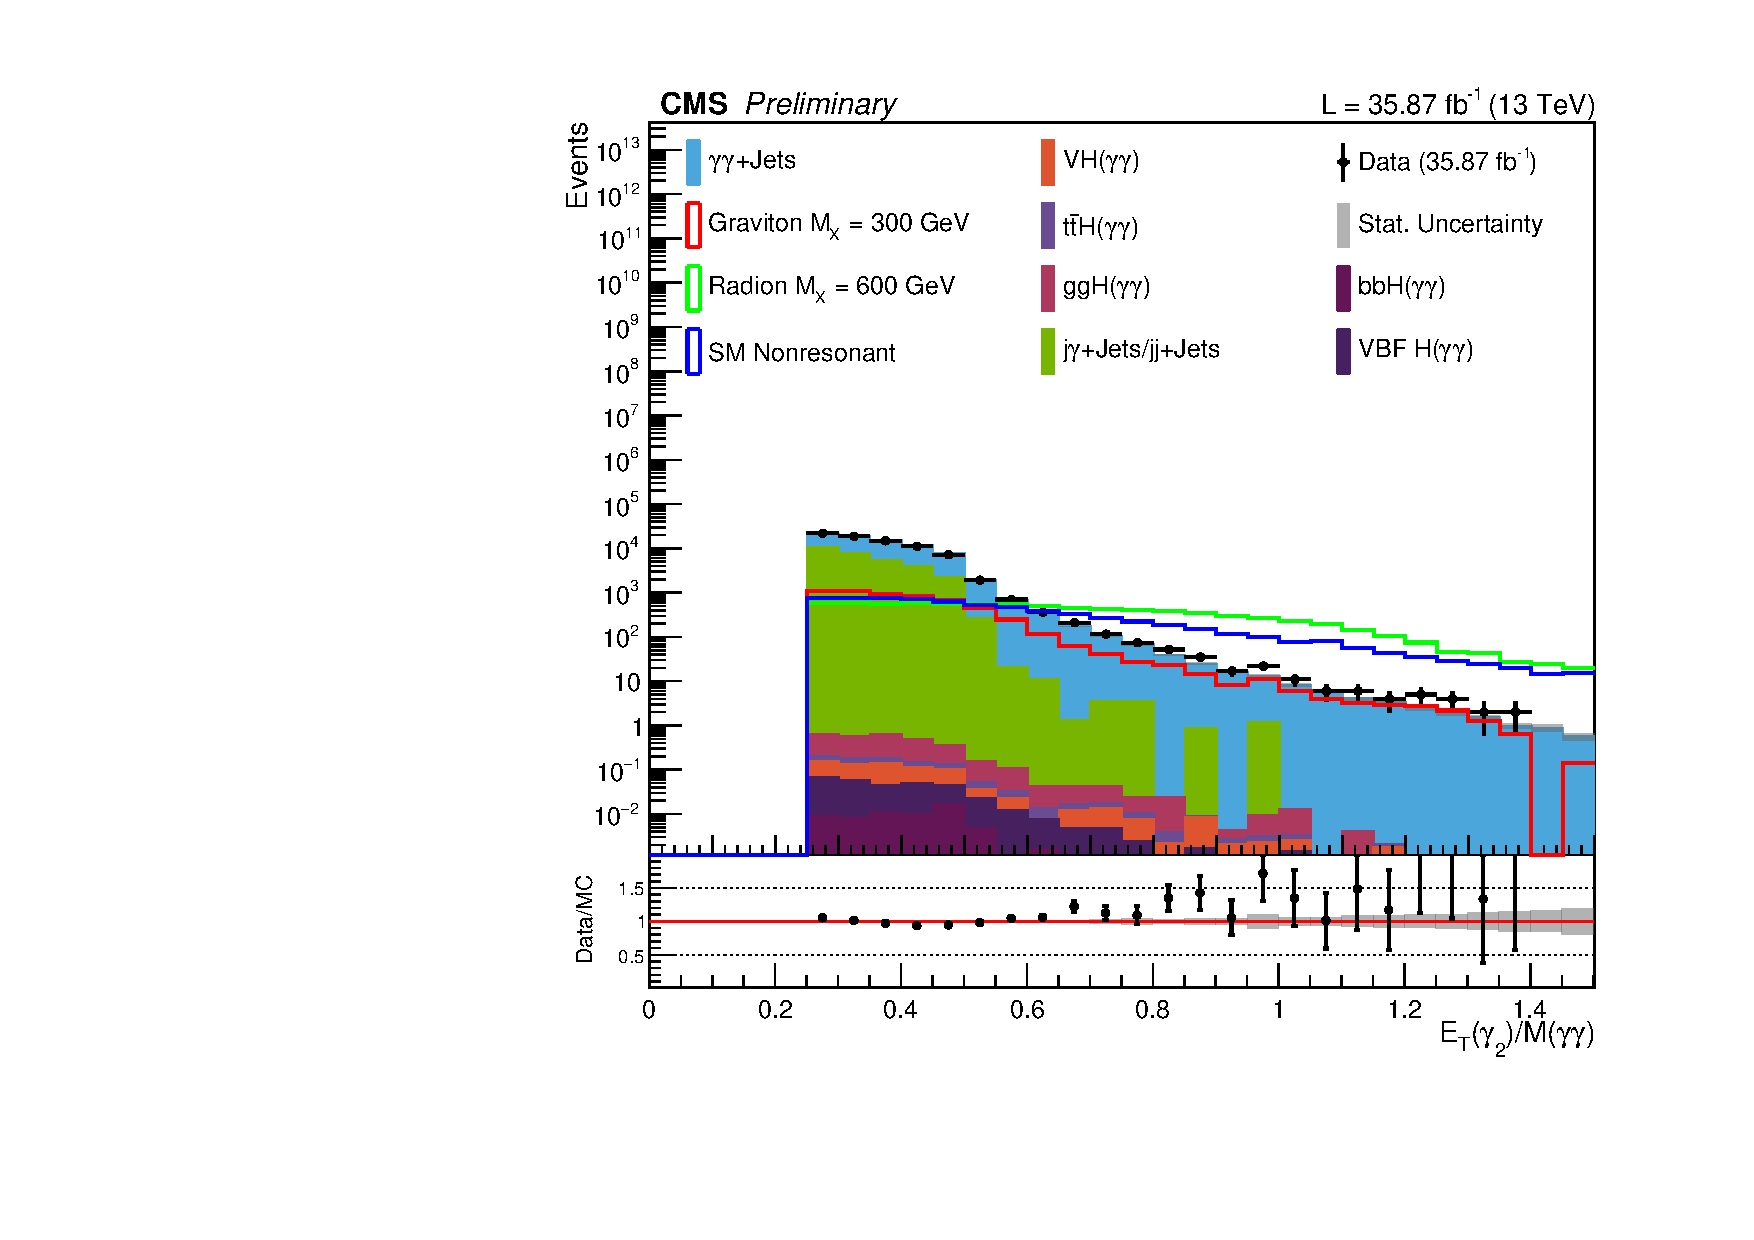
\includegraphics[width=0.45\textwidth]{figures/sec-control/LOG_sphoptmgg}\hfil
  \caption{Distributions for the blinded signal region.}
\label{fig:cp_mgg7}
\end{figure*}

